\begin{figure*}[t]
    \centering
    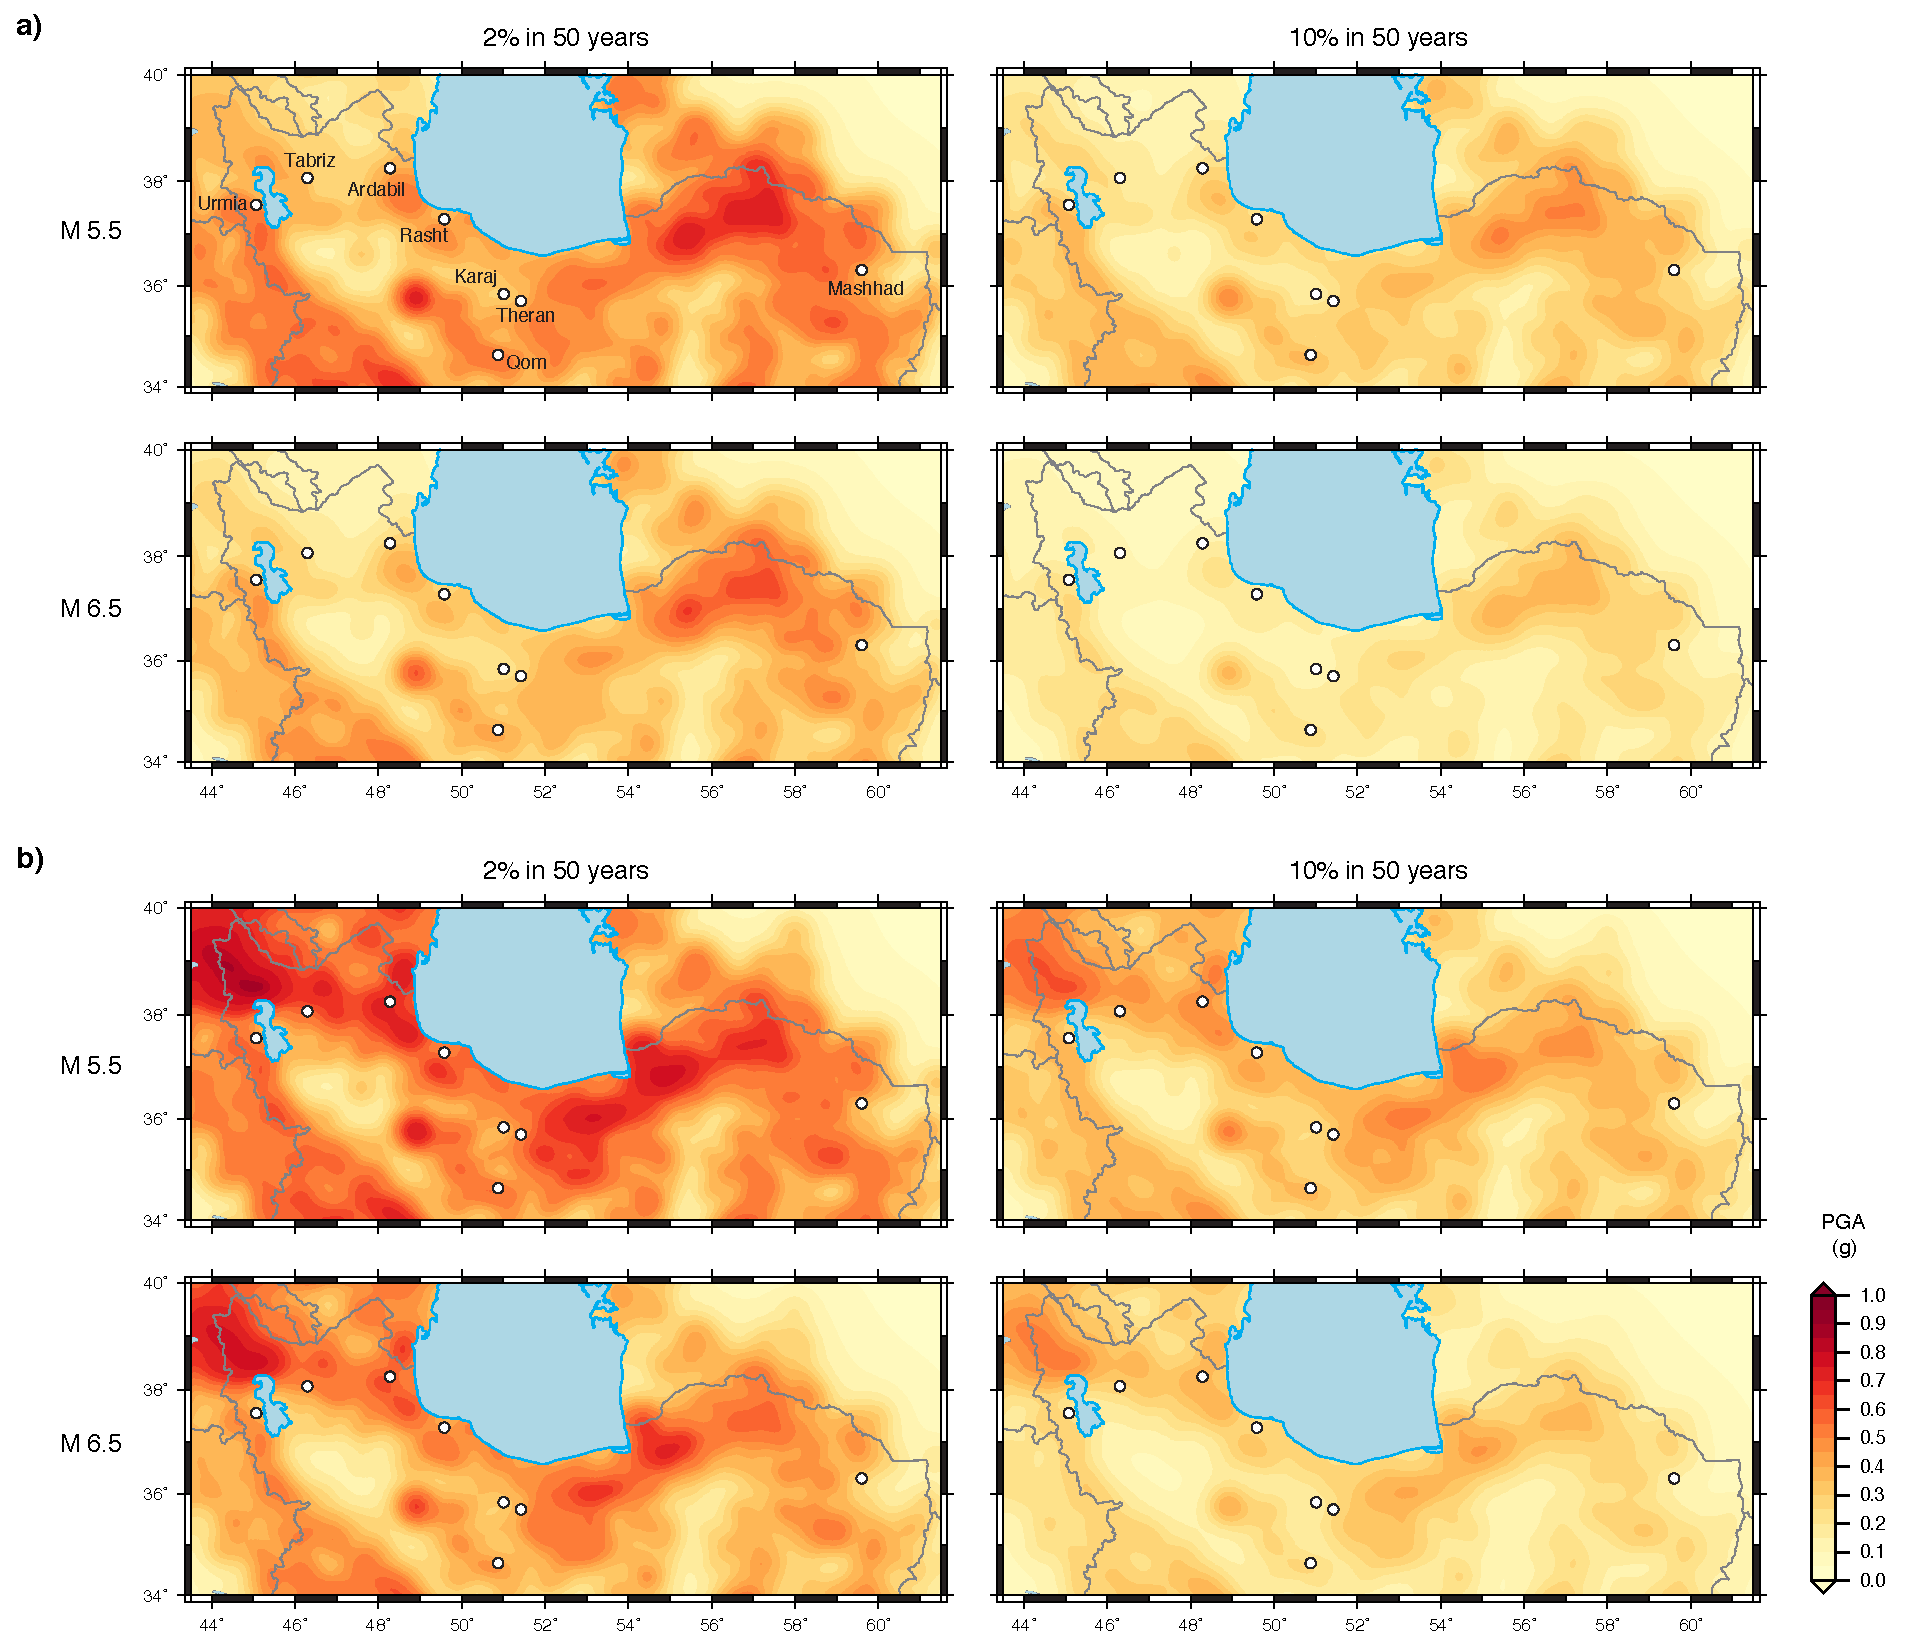
\includegraphics[width=\textwidth]{figures/pdf/figure-08.pdf} 
    \caption{Expected mean peak ground acceleration (PGA) for 2 and 10 percent of probability of exceeding earthquake magnitudes $M_w$ 5.5 and 6.5 for (a) the five seismic regions R model and (b) the uniform seismic region U model.}
    \label{fig:pga}
\end{figure*}

\begin{figure*}[t]
    \centering
    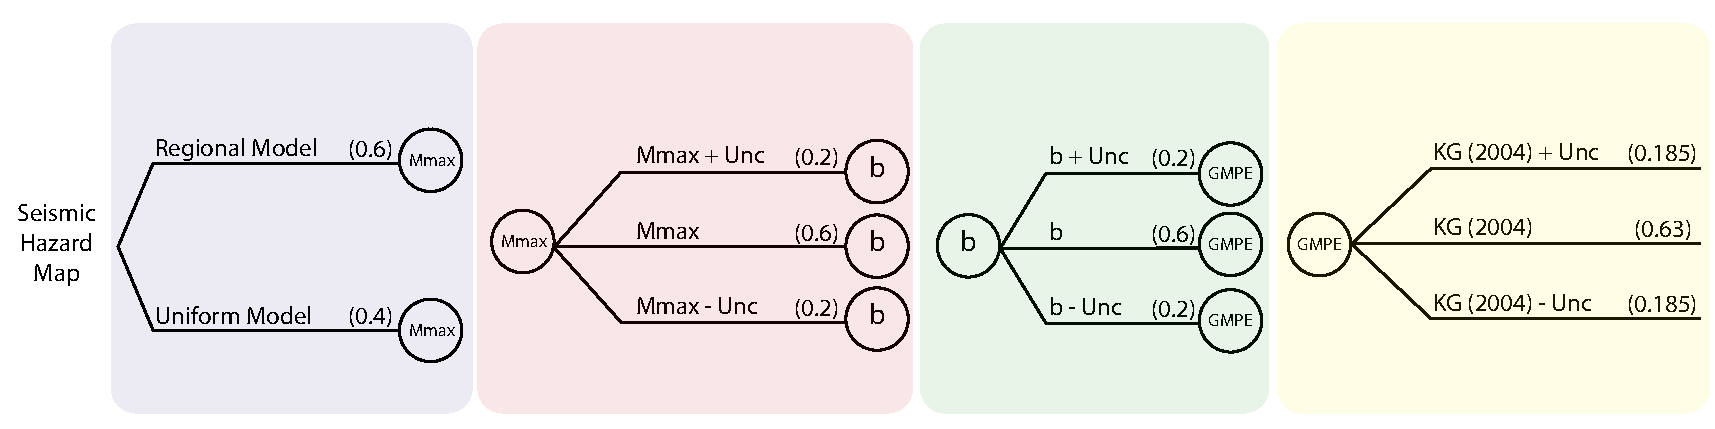
\includegraphics[width=\textwidth]{figures/pdf/figure-09.pdf} 
    \caption{Difference between the mean PGA values obtained for the uniform U model results and the corresponding R models for 2 (left) and 10 (right) percent probabilities of exceeding magnitudes $M_w$ 5.5 (top) and 6.5 (bottom).}
    \label{fig:pgadiff}
\end{figure*}

\begin{figure*}[t]
    \centering
    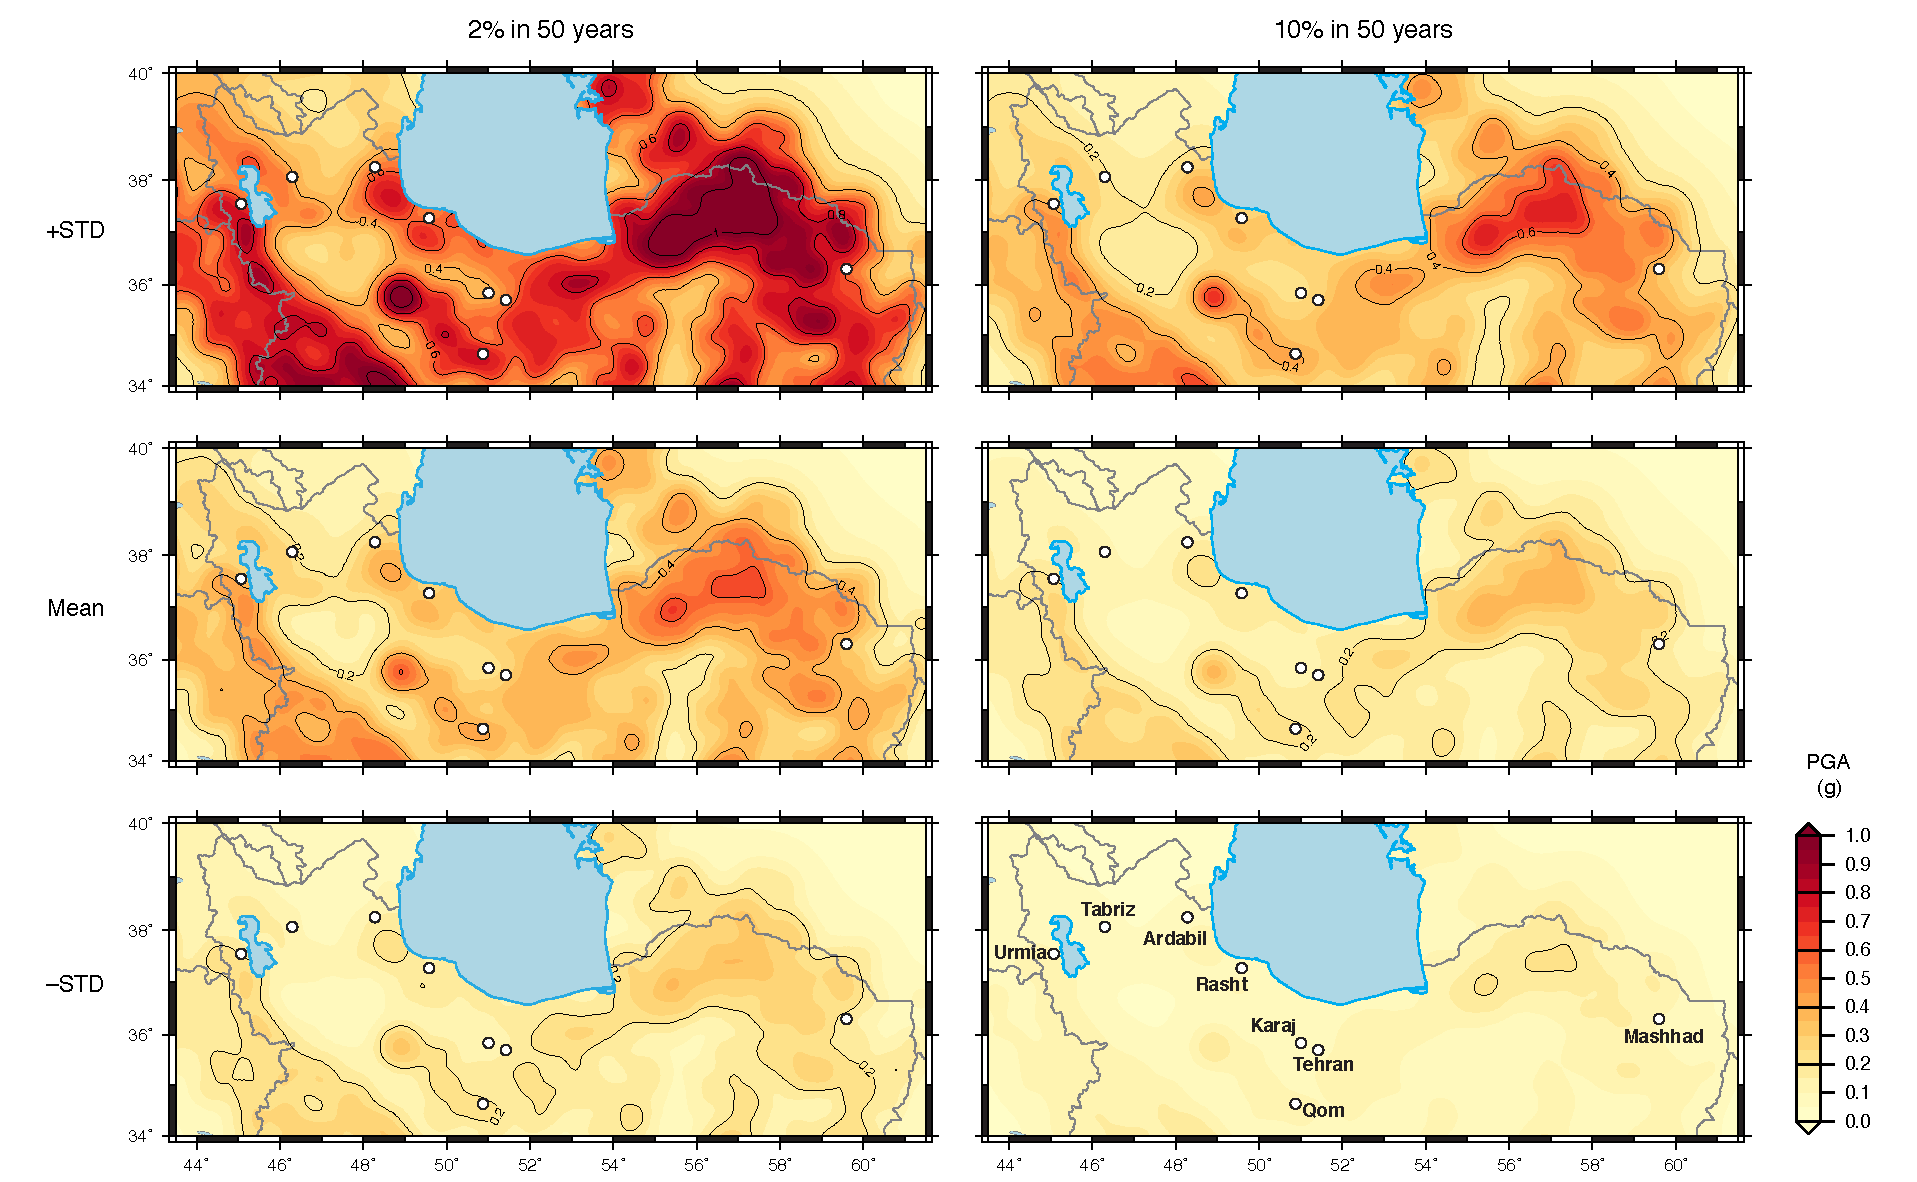
\includegraphics[width=\textwidth]{figures/pdf/figure-10.pdf} 
    \caption{plus minus std for M6.5.}
    \label{fig:pgastd}
\end{figure*}

\section{Results and Analysis}

Using the data, parameters, and procedures described above, we considered different hazard models based on whether we use the five distinct seismic hazard regions or the whole area of interest as a uniform seismic hazard region. We call these the R and U models, respectively. We also considered two threshold levels of ground motion for events exceeding magnitudes $M_w$ 5.5 and 6.5. We refer to these models with the suffixes 5.5 and 6.5, respectively. Each of these are considered under two probabilities of exceedance, at 2 and 10 percent in 50 years, for which we use the prefixes 2 and 10, respectively. These probabilities correspond to return periods of 475 and 2475 years. As an example of the chosen nomenclature, we refer to the results for 2 percent probability of exceeding an event magnitude $M_w$ 5.5 in 50 years under the five seismic regions model as the 2R5.5 model results.

In the distinct regions R models, we computed the probability of exceedance of the ground motion separately for each region and then add them together in order to have the contribution of all regions for any given grid point within the region of interest. The results are obtained in the form of annual rate of exceedance. Expected PGA values are therefore a slice of the actual hazard curves cut across all grid points for a chosen magnitude.

We extract expected levels of ground motion for magnitudes 5.5 and 6.5, based on the assumption that buildings of different construction systems may be vulnerable to different magnitude earthquakes. It is natural to anticipate that modern constructions in urban areas in Iran follow current building regulations and are thus well-designed to withstand moderate magnitude earthquakes $M_w$ 4.5--6.5, and to undergo moderate non-life threatening damage during $M_w > 6.5$ events. Unconventional constructions in poor city outskirts, rural housing and historical buildings may, however, be vulnerable to $M_w \leq 5.5$, and thus becomes relevant to entertain lower magnitude exceedance levels. In turn, the 2 and 10 percent probability of exceedance in a 50-years span are considered a standard practice in seismic design \citep[e.g.,][]{BHRC2014}.

Fig.~\ref{fig:pga} shows the expected mean PGA values obtained using the selected attenuation relationship as a measured of gravity (g) throughout the region of interest for the different model combinations. As can be expected, the highest levels of ground motion are associated with the 2R5.5 and 2U5.5 models, and the lowest with the 10R6.5 and 10U6.5 models. In results for the R models shown Fig.~\ref{fig:pga}a, the highest levels of expected ground motion occur in the Kopeh Dagh region along the border with Turkmenistan, followed by ground motions in the north-central region west from Tehran and Karaj, and in the vicinity of the Piranshahr fault between the Zagros and Azerbaijan seismic regions (see Fig.~\ref{fig:selected}b for reference). The Azerbaijan seismic zone does not present equally high levels of expected ground motion. In the U models shown in Fig.~\ref{fig:pga}b, on the other hand, the highest levels of expected ground motion are observed precisely in the area corresponding to the Azerbaijan seismic region, especially in the vicinity of the North Tabriz Fault system (see Fig.~\ref{fig:selected} for reference).

In general, the U models exhibit higher levels of expected ground motions when compared to their corresponding R models. This is illustrated in Fig.~\ref{fig:pgadiff}, which shows the differences between both set of models, U--R (U minus R). In this figure, positive values indicate that the U models have larger mean PGA values than the R models. As it can be seen, this is true practically throughout the whole region at very low levels, and in particular in the north-central region at a moderate level of up to 0.2 g and most predominantly in the north-western region of Azerbaijan at levels of about 0.2 to 0.5 g.

Overall, these results are consistent with the seismicity observed in Fig.~\ref{fig:catalog}. The R model results, however, seem to be more sensitive to the influence of large magnitude events observed in both the historical and modern seismicity maps, with concentration of strong earthquakes in the Alborz and Kopeh Dagh regions; whereas the U model results seem to be more sensitive to the influence of low-to-moderate magnitude events, especially in the Azerbaijan region. This may be the cause of 

These, of course, are only mean expected levels of ground motion. A more complete picture is captured when considering statistical deviations. Fig.~\ref{fig:pgastd} shows again the mean PGA for the models 2R6.5 and 10R6.5, but this time along with the marginal values of plus and minus one standard deviation. Here, the standard deviation is carried forward in the calculation from the attenuation relationship and thus affects every grid point differently depending on the added contributions from each region. 

The highest expected PGA values are observed in the 2R6.5+STD model with accelerations of higher than 1 g in the Kopeh Dagh region and west of Tehran, and 0.8 g south of the North Tabriz Fault system and in the Zagros region along. These maximum values should, nonetheless, be interpreted with caution given the fact that predictions are based on rock-site assumptions and do not include any kind of site effects, such as inelastic deformation of near-surface geotechnical layers which may often contribute to mitigate peak accelerations.

An additional consideration to make here is the fact that one cannot claim any of the models to be uniquely correct. They all carry a certain level of epistemic uncertainty which make them equally accurate and inaccurate at the same time. An means to reduce the overall uncertainty intrinsically associated with each model is to use combinations of different models. We consider two types of combinations here to aid our analysis. First, we combine results at both magnitude thresholds following the hypothesis that in areas were mixed reinforced and unreinforced buildings are present, the hazard and associated expected ground motions will be an average of both models, i.e. $frac{1}{2}(5.5+6.5)$. Second, we consider a combination of the five-regions model and the uniform model, i.e. $frac{1}{2}(\mathrm{U}+\mathrm{R})$, based on the hypothesis that both models carry forward valid information about the local and regional seismicity.

Fig.~\ref{fig:}a shows 

~\\
* * *
\\

% \subsection{Hazard Curve}

% We calculated the probability of exceedance of the ground motion from different ground motion levels, separately for each of 5 regions. 
% We add the probability of all regions in order to have the effect of seismicity from all tectonic seismic regions. 
% The results are presented as annual rate of exceedance. 

Fig.~\ref{fig:hazardcurve} represents the hazard curve of different model for some of important northern cities in Iran. 

\begin{figure*} [!ht]
\centering
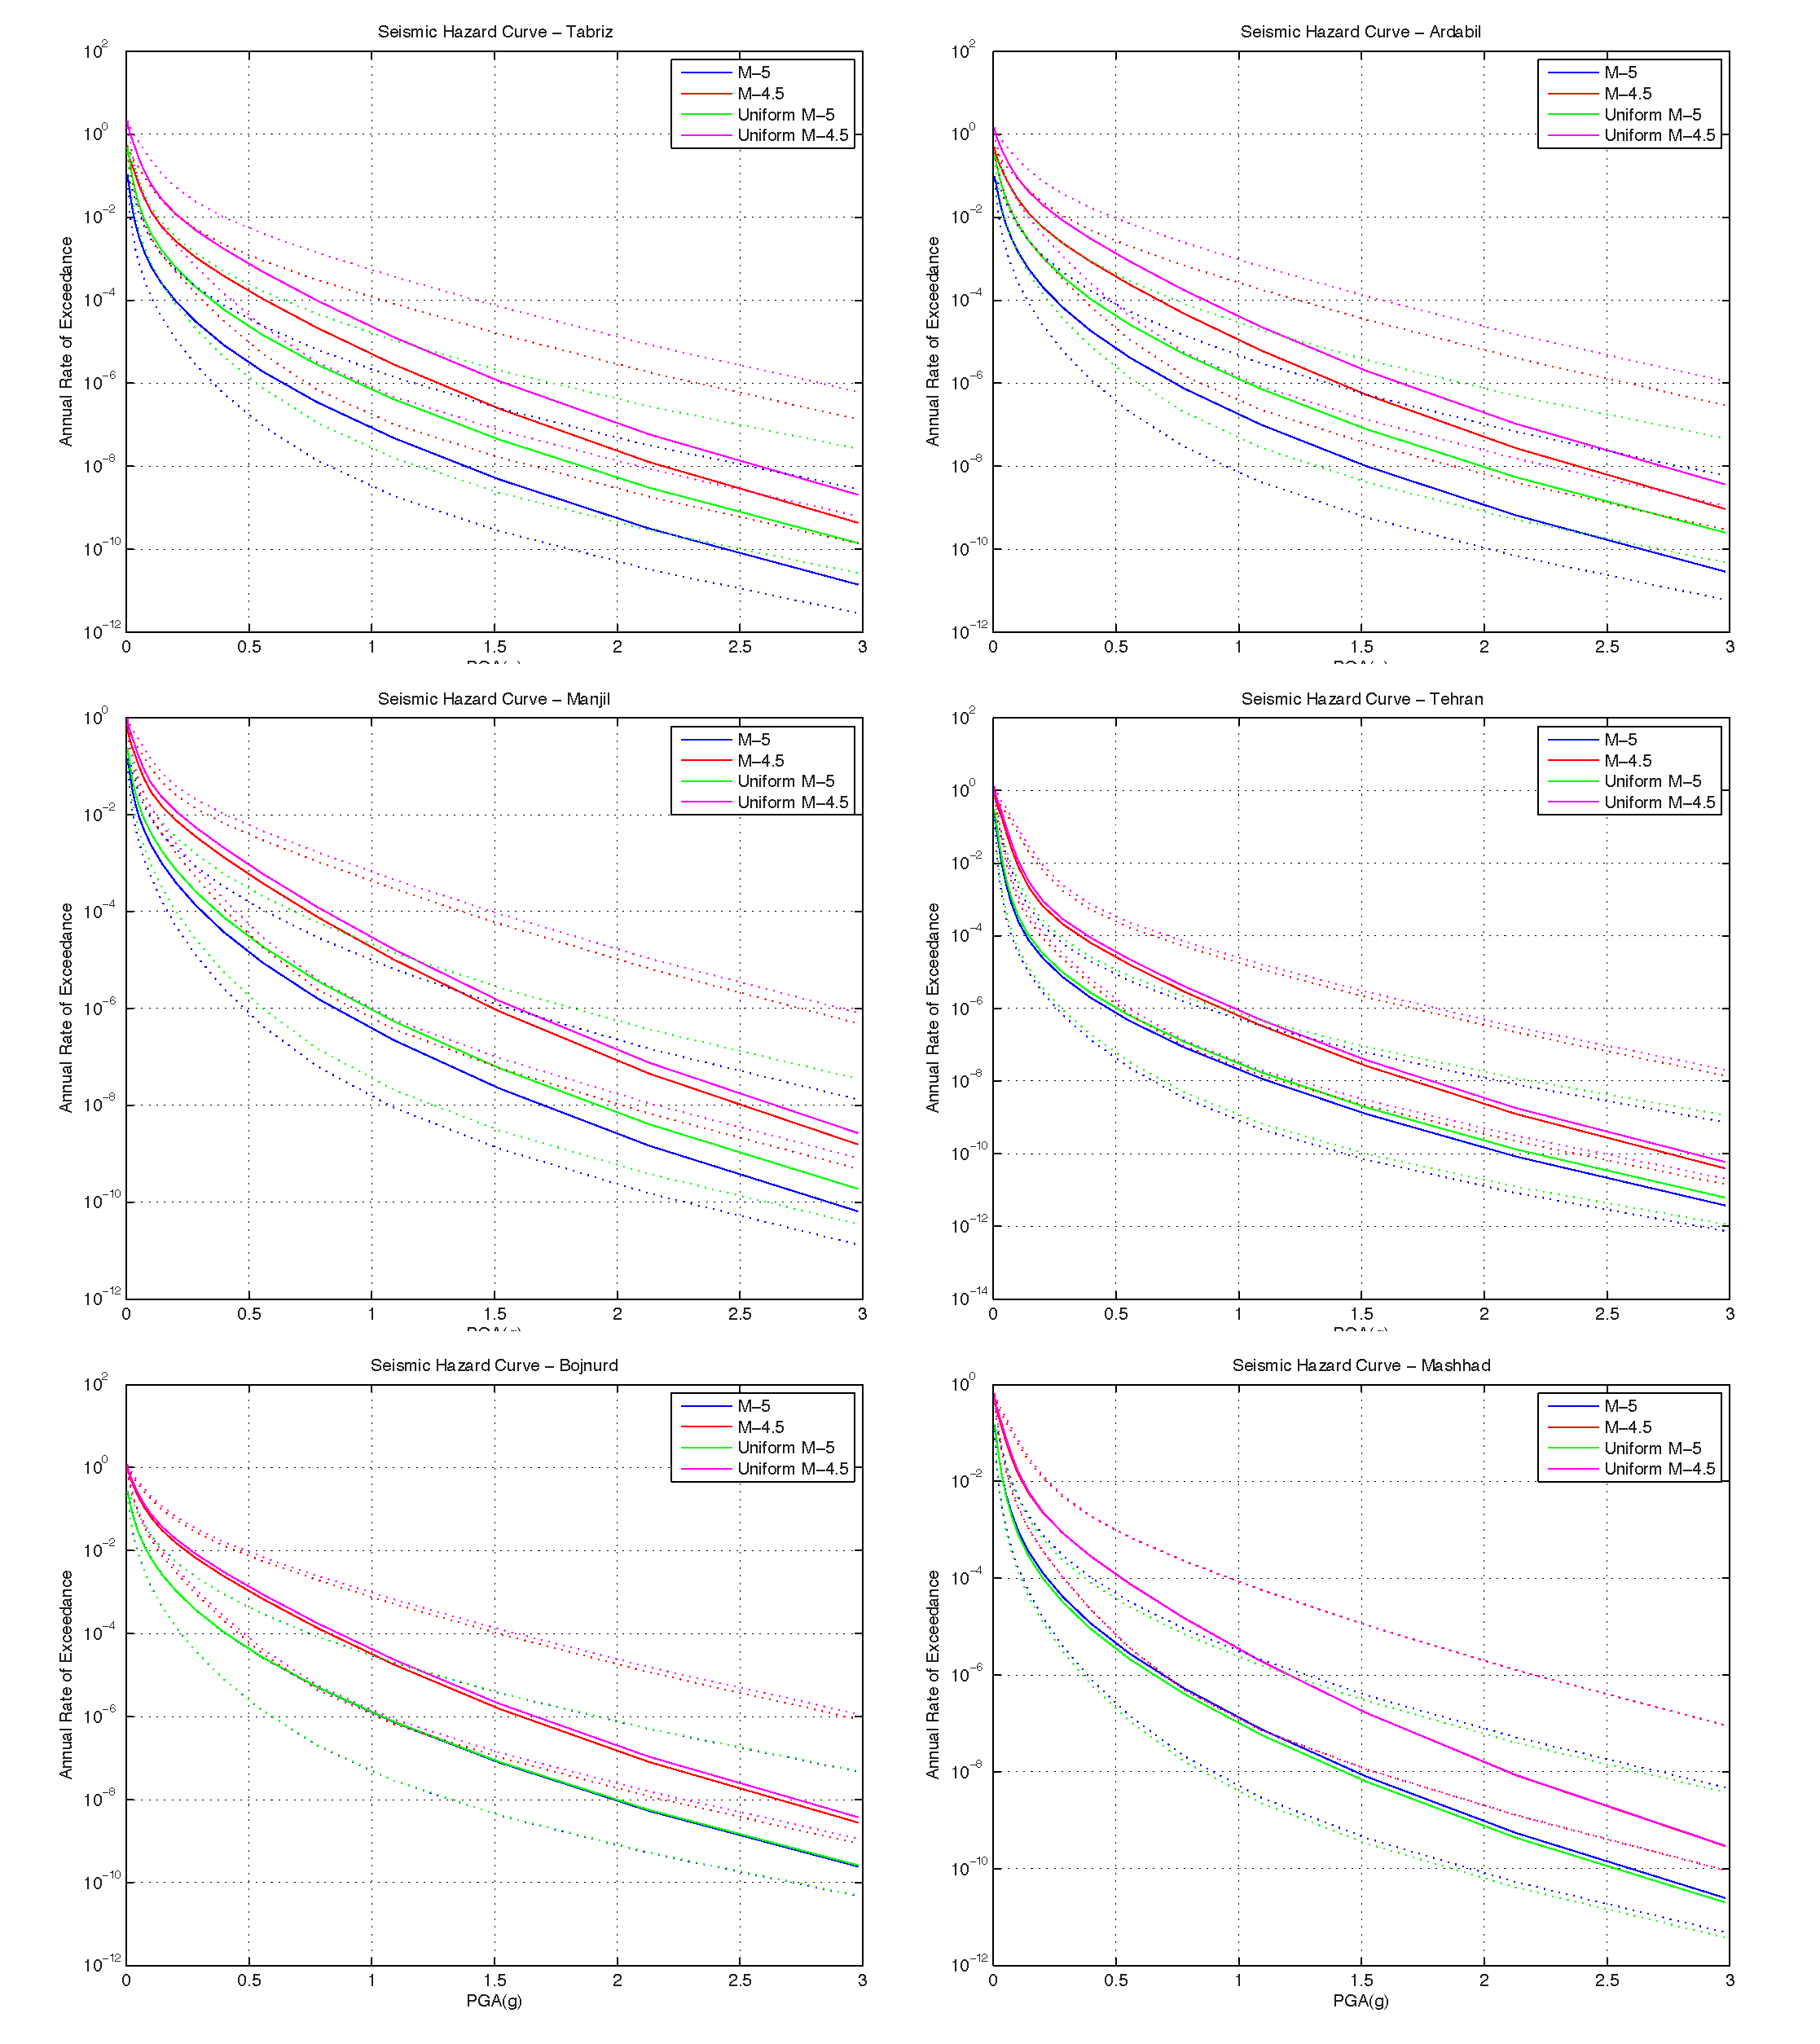
\includegraphics[scale=0.4]{figures/pdf/HazardCurve.pdf} 
\caption{Seismic Hazard Curve of Northern Cities in Iran}
\label{fig:hazardcurve}
\end{figure*}

% \subsection{Peak Ground Acceleration}

We pick the peak ground acceleration for 10\% and 2\% probability of exceedance in 50 years which correspond with 0.002 and 0.0004 annual rate of exceedance. 

% Fig.~\ref{fig:pga_10_mean} and Fig.~\ref{fig:pga_2_mean} show the results for 10\% and 2\% probability of exceedance in 50 years, respectively.
% These results are according to the mean value of the attenuation relationship.
% Fig.~\ref{fig:pga_10_mean_uniform} and Fig.~\ref{fig:pga_2_mean_uniform} show the results for 10\% and 2\% probability of exceedance in 50 years for the uniform model, respectively.

% -------

% Even though in this study we are interested in investigating seismic hazard study in the northern Iran, in the smoothed seismicity method we defined the border of the study region broadly enough to ensure that the seismicity outside of the border doesn't affect the study area.  
% In addition, the border of the influenced area should surround the area of interest as uniformly as possible \citep{Lapajne1997}. 
% Therefore, our study region includes parts of central and eastern Iran and the Zagros tectonic seismic regions.

% We calculated the $a-values$ for each cell and spatially smoothed over a grid of $0.1 \times 0.1$ in latitude and longitude. 
% We assume magnitude increment as $\Delta_M = 0.1$. 

% In this model, events are not assigned to specific faults and are assumed to be potential seismogenic sources, and are spatially gridded to cells.

% Different correlation distances have been used in different studies, which are generally dependent on the accuracy of the location of the recorded earthquakes. \citet{Frankel1995} and \citet{Boyd2008} assumed the correlation distance to be 50 $km$. \citet{Barani2007} used distance of 25 $km$ based on previous studies that suggested the correlation function of the Alps and Apennines in Italy. \citet{Foteva2006} used 10 and 15 km in a different model. Correlation distance is a very sensitive parameter in smoothed seismic hazard maps, and it is a factor of uncertainty in earthquake location. In the Iranian earthquake catalog, the magnitude uncertainties were assumed to be in the interval of $\pm$ 0.25 magnitude units and epicentral errors of $\pm$ 30 km \citep{Zare2012}. Even though these error margins are different for different events in terms of instrumental or historical events, in this study we assumed the correlation distance as 30 km because of the lack of knowledge about other historical events. 

% Regarding the study domain and the 0.1 grid size, the total number of source is grid sites is 11651. Even though \citet{Kalkan2004} derived the attenuation relationship up to 250 km, since \citet{Zafarani2014} used data up to 200 km to evaluate the GMPEs, we set the model to compute the ground motions at distances of less than 200 km.

% Fig.~\ref{fig:10percent} and Fig.~\ref{fig:2percent} show the seismic hazard map based on background seismicity for 10\% and 2\% probability of exceedance in 50 years, respectively. The areas of large probabilistic ground motions clearly coincide with zones with a large number of events with magnitude 3 and larger.

% ==================
% OLD STUFF NOT USED
% ==================

% Regarding the study domain and the 0.1 grid size, the total number of source as grid points is 13561. 

% corresponding to return periods of 475 and 2475 years.